% Copyright 2005-2016 Airbus-EDF-IMACS-Phimeca
% Permission is granted to copy, distribute and/or modify this document
% under the terms of the GNU Free Documentation License, Version 1.2
% or any later version published by the Free Software Foundation;
% with no Invariant Sections, no Front-Cover Texts, and no Back-Cover
% Texts.  A copy of the license is included in the section entitled "GNU
%  Free Documentation License".
\renewcommand{\etapemethodo}{B}
\renewcommand{\nomfichier}{docref_B21_MaximumLikelihood}
\renewcommand{\titrefiche}{Maximum Likelihood Principle}

\Header

\MathematicalDescription{

  \underline{\textbf{Goal}} \vspace{2mm}

  This method deals with the parametric modelling of a probability distribution for a random vector $\vect{X} = \left( X^1,\ldots,X^{n_X} \right)$. The appropriate probability distribution is found by using a sample of data $\left\{ \vect{x}_1,\ldots,\vect{x}_N \right\}$. Such an approach can be described in two steps as follows:
  \begin{itemize}
  \item Choose a probability distribution (e.g. the Normal distribution, or any other distribution available in OpenTURNS see \otref{docref_B121_DistributionSelection}{standard parametric models}),
  \item Find the parameter values $\vect{\theta}$ that characterize the probability distribution (e.g. the mean and standard deviation for the Normal distribution) which best describes the sample $\left\{ \vect{x}_1,\ldots,\vect{x}_N \right\}$.
  \end{itemize}

  The maximum likelihood method is used for the second step.
  \vspace{2mm}

  \underline{\textbf{Principle}} \vspace{2mm}

  In the current version of OpenTURNS this method is restricted to the case where $n_X = 1$ and continuous probability distributions. Please note therefore that $\vect{X} = X^1 = X$ in the following text.
  The maximum likelihood estimate (MLE) of $\vect{\theta}$ is defined as the value of $\vect{\theta}$ which maximizes the likelihood function $L\left(X,\vect{\theta}\right)$:
  \begin{align*}
    \hat{\vect{\theta}} = \textrm{argmax}\ L\left(X,\vect{\theta} \right)
  \end{align*}

  Given that $\left\{x_1,\ldots,x_N \right\}$ is a sample of independent identically distributed (i.i.d) observations, $L\left(x_1,\ldots, x_N, \vect{\theta} \right)$ represents the probability of  observing such a sample assuming that they are taken from a probability distribution with parameters $\vect{\theta}$. In concrete terms, the likelihood $L\left(x_1,\ldots, x_N, \vect{\theta}\right)$ is calculated as follows:

  \begin{displaymath}
    L\left(x_1,\ldots, x_N, \vect{\theta} \right) = \prod_{j=1}^{N} f_X\left(x_j;\vect{\theta} \right)
  \end{displaymath}
  if the distribution is continuous, with density $f_X\left(x;\vect{\theta}\right)$.

  For example, if we suppose that $X$ is a Gaussian distribution with parameters $\vect{\theta}= \{ \mu,\sigma \}$  (i.e. the mean and standard deviation),
  \begin{eqnarray*}
    L\left(x_1,\ldots, x_N, \vect{\theta}\right) &=& \prod_{j=1}^{N} \frac{1}{\sigma \sqrt{2\pi}} \exp \left[ -\frac{1}{2} \left( \frac{x_j-\mu}{\sigma}  \right)^2  \right] \\
    &=& \frac{1}{\sigma^N (2\pi)^{N/2}} \exp \left[ -\frac{1}{2\sigma^2} \sum_{j=1}^N \left( x_j-\mu \right)^2  \right]
  \end{eqnarray*}
  The following figure graphically illustrates the maximum likelihood method, in the particular case of a Gaussian probability distribution.

  \begin{center}
    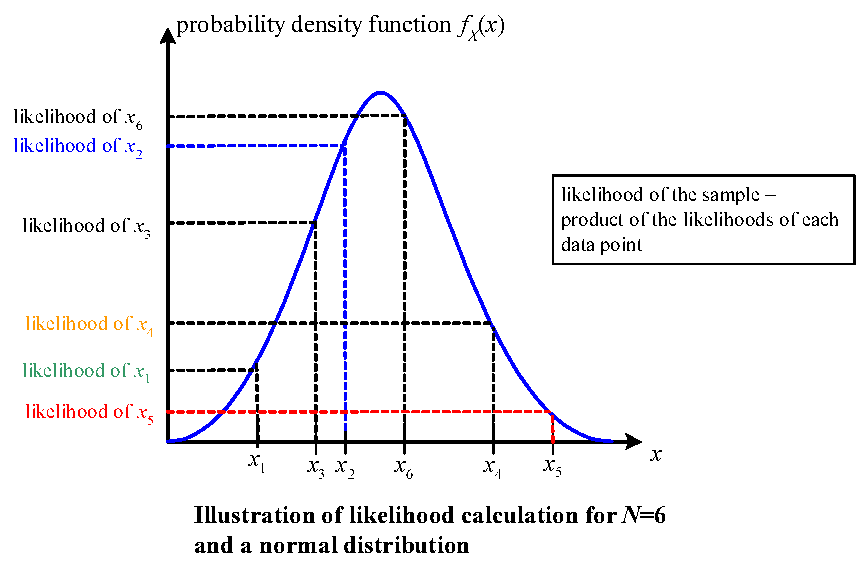
\includegraphics[scale=0.8]{Figures/MV.pdf}
  \end{center}

  In general, in order to maximize the likelihood function classical optimization algorithms (e.g. gradient type) can be used. The Gaussian distribution case is an exception to this, as the maximum likelihood estimators are obtained analytically:
  \begin{align*}
    \widehat{\mu}  = \frac{1}{N} \sum_{i=1}^N x_i,\ \widehat{\sigma^2} = \frac{1}{N} \sum_{i=1}^N \left( x_i - \widehat{\mu} \right)^2
  \end{align*}

}
{
  -
}


\Methodology{
  Having specified the variable of interest and having defined a criterion (step A "Specifying Criteria and the Case Study"), the uncertainty of the input variable $X^i$ must be then quantified in step B. The superscript $i$ is omitted, as only a single component is used here, that is a single unknown variable (or source of uncertainty).\\

  \textbf{Input:}

  $\left\{x_1,\ldots,x_N \right\}$: sample data

  \textit{Distribution}: Distribution type chosen from the proposed continuous 1-dimensional distributions in \otref{docref_B121_DistributionSelection}{standard parametric models}\\


  \textbf{Output :}

  $\hat{\vect{\theta}}$: maximum likelihood estimate of $\vect{\theta}$
}
{
  The sample size used in the maximum likelihood method has an effect on the quality of results. In fact:

  \begin{itemize}
  \item as $N$ tends to infinity, the asymptotic theory results assure, under certain assumptions concerning the regularity of the model, that the MLE is the best possible estimator (its bias tends towards 0 i.e. no tendency towards under- or over-estimation, the uncertainty of  $\hat{\vect{\theta}}$ is lesser than in all other unbiased estimation methods); in practice, one often considers the asymptotic behaviour to be reached when $N \geq$ a few dozens, even if no theoretical rule can assure this with certitude.
  \item if $N$ is smaller, the MLE is still useful but $\hat{\vect{\theta}}$ is less robust (uncertainty greater and bias possible).
  \end{itemize}

  A more advanced study of the goodness-of-fit of the selected probability distribution with the given sample data is described in \otref{docref_B221_Graph}{Graphical analysis} \otref{docref_B222_TestKS}{Kolmogorov-Smirnov test}, \otref{docref_B222_TestCVM}{Cramer-Von Mises test}, \otref{docref_B222_TestAD}{Anderson-Darling test} and \otref{docref_B222_BayesianInformationCriterion}{BIC criterion}.

  The following bibliographical references provide main starting points for further study of  this method:
  \begin{itemize}
  \item Saporta G. (1990). "Probabilités, Analyse de données et Statistique", Technip
  \item Dixon W.J. \& Massey F.J. (1983) "Introduction to statistical analysis (4th ed.)", McGraw-Hill
  \end{itemize}
}
